\documentclass{article}
\usepackage{main}

\title{Al-Khwarizmi}
\date{12 Novembre 2024}
\author{Première Spécialité Mathématiques}

\begin{document}
\maketitle

Le texte suivant est une retranscription d'un texte attribué à \emph{Al-Khwarizmi}, savant bagdadi né dans les années $780$.

\begin{quote}
\og J'ai rédigé sur le sujet (\dots) un livre abrégé englobant les choses les plus subtiles et les plus nobles du calcul dont ont besoin les gens dans leurs héritages, dans leurs donations, dans leurs partages, dans leurs jugements, dans leurs commerces et dans toutes les transactions qu'il y a entre eux à propos de l'arpentage des terres, du creusement des canaux, de la géométrie et d'autres choses relatives à ses aspects et à ses arts (\dots). J'ai découvert ainsi que les nombres dont on a besoin dans le calcul sont de trois types : ce sont les racines, les biens et le nombre seul \dots \fg
\end{quote}

\section{Traduction}
En algèbre, Al-Khwarizmi considère plusieurs sortes de nombres : les nombres simples ou dirhams (de la drachme, monnaie grecque), les racines, les biens qui sont les produits de racines par elles-mêmes. Dans la suite on dira parfois nombre au lieu de dirham. Retranscrire sous forme classique les équations suivantes telles que présentées par Al-Khwarizmi.

\begin{enumquestions}
\item \og Tout bien tel que si on lui ajoute vingt et un dirham, la somme qui en résulte est dix racines de ce bien.\fg
\item \og Un bien et dix de ses racines égalent trente-neuf dirhams \fg
\end{enumquestions}

\emptybox{2cm}

\section{Résolution}
Concernant la résolution de \og Un bien et dix de ses racines égalent trente-neuf dirhams \fg, Al-Khwarizmi propose le procédé de résolution suivant :

\begin{quote}
\og Son procédé de résolution consiste à diviser le nombre de ses racines par deux, et c'est cinq dans ce problème. Tu le multiplies par lui-même et ce sera vingt-cinq. Tu l'ajoutes à trente-neuf. Cela donnera soixante-quatre. Tu prends alors sa racine carrée qui est huit et tu en retranches la moitié du nombre des racines et c'est cinq. Il reste trois et c'est la racine du bien que tu cherches et le bien est neuf. \fg
\end{quote}

\begin{enumquestions}
\item Quelle est la solution apporté par Al-Khwarizmi après sa résolution ?
\item Décrire les étapes de l'algorithme de résolution d'Al-Khwarizmi.
\item S'inspirer de la méthode d'Al-Khwarizmi pour résoudre l'équation suivante : $x^2 + 8x = 33$.
\end{enumquestions}
\newpage

\emptybox{8cm}

\section{Preuve}

La preuve de correction de son algorithme a été apportée par Al-Khwarizmi lui-même. Il s'agit d'une preuve géométrique consistant à représenter les données du problème sous forme géométrique.

\begin{center}
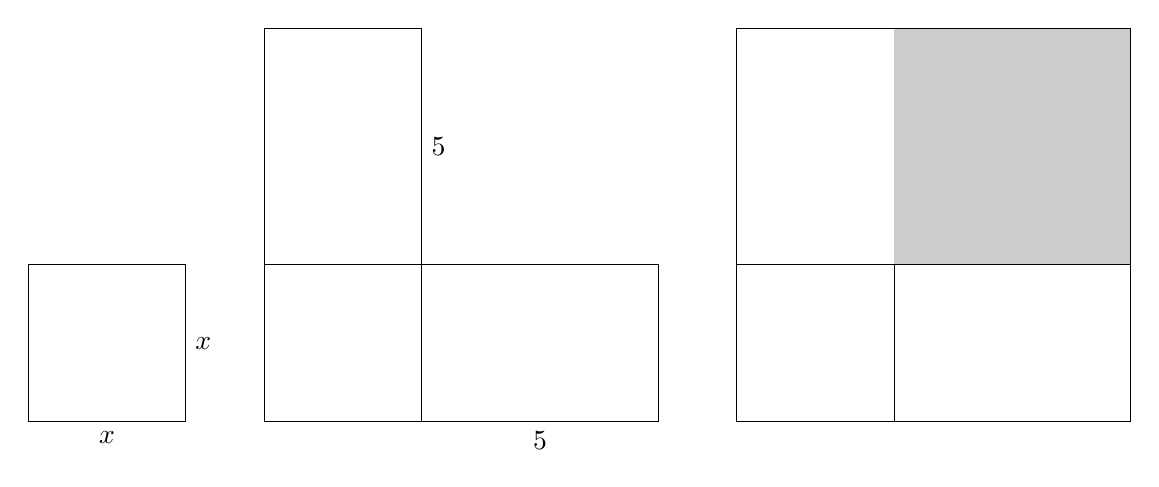
\begin{tikzpicture}
\draw (0,0) -- (2,0) node[midway, below] {$x$} -- (2,2) node[midway, right] {$x$} -- (0,2) -- cycle;
\begin{scope}[xshift=3cm]
\draw (0,0) -- (2,0) -- (2,2) -- (0,2) -- cycle;
\draw (2,0) -- (5,0) node[midway, below] {$5$} -- (5,2) -- (2,2);
\draw (2,2) -- (2,5) node[midway, right] {$5$} -- (0,5) -- (0,2);
\end{scope}
\begin{scope}[xshift=9cm]
\draw (0,0) -- (2,0) -- (2,2) -- (0,2) -- cycle;
\draw (2,0) -- (5,0) -- (5,2) -- (2,2);
\draw (2,2) -- (2,5) -- (0,5) -- (0,2);
\fill[color=gray!40] (2,2) -- (5,2) -- (5,5) -- (2,5);
\draw (2,2) -- (5,2) -- (5,5) -- (2,5);
\end{scope}
\end{tikzpicture}
\end{center}
\begin{enumerate}
\item On considère un carré de côté $x$ (le \og bien \fg);
\item On borde ce carré de deux rectangles de largeur $x$ et de longueur $\dfrac{10}{2}$ (la moitié des \og racines \fg)
\item On complète la figure pour obtenir un carré. 
\end{enumerate}

\begin{enumquestions}
\item Quelle est l'aire de la figure non-grisée, en fonction de $x$ ?
\item Sachant qu'un \og bien et dix de ses racines égalent trente-neuf dirhams \fg, quelle est l'autre valeur de cette aire ?
\item Quelle est l'aire de la partie grisée ? En déduire l'aire du carré obtenue à la fin de l'étape $3$.
\item En déduire que résoudre l'équation initiale revient à résoudre $(x+5)^2 = 64$.
\item Proposer alors une solution de l'équation.
\item Est-ce la seule solution possible de cette équation sur $\R$ ? Pourquoi la résolution d'Al-Khwarizmi ne renvoie-t-elle qu'une seule solution d'après vous ?
\end{enumquestions}

\end{document}